%******************************************************************
\section{Statistical Framework}\label{sec:bc_statistical_framework}
%******************************************************************

% Introductory Paragraph
The calibration framework in this thesis is in line with the seminal work of Kennedy and O'Hagan \cite{Kennedy2001};
which is widely adapted in the applied literature \cite{Bayarri2007,Higdon2008,Arendt2012,Reichert2012,Higdon2013}.
\marginpar{Calibration framework}
Meanwhile, its explicit formulation uses a set of notations adapted from different sources \cite{Kennedy2001,Santner2003,Huard2006,Reichert2012,Wicaksono2016}.
Suppose an experiment on a physical system is being conducted and, in parallel to that, a computer simulator of the system is available.
Let $y_E$ be the experimental observation of the system response (i.e., the \glsfirst[hyper=false]{qoi}) taken at \emph{controllable} inputs $\bm{x}_c$,
then its relationship to the true \emph{unknown} response value $y_T$ is given by
\begin{equation}
    y_E(\bm{x}_c, \bm{\lambda}) = y_T (\bm{x}_c, \bm{\lambda}) + \epsilon(\bm{\lambda})
\label{eq:bc_observation_true}
\end{equation}
where $\epsilon$ is an observation error;
and $\boldsymbol{\lambda}$ is an element of an observation layout $\boldsymbol{\Lambda}$ detailed below.
The true value, in turn, is linked to the prediction made by the computer simulator $y_M$ by
\begin{equation}
    y_T(\bm{x}_c, \boldsymbol{\lambda}) = y_M (\bm{x}_c, \hat{\bm{x}}_m, \boldsymbol{\lambda}) + \delta (\bm{x}_c, \boldsymbol{\lambda})
\label{eq:bc_true_simulation}
\end{equation}
where $\delta$ is the \emph{model bias}, defined as the difference between the true response value and the simulator prediction made by using $\hat{\bm{x}}_m$, the best (``true'') value of the \emph{model} parameters.
\marginpar{Model bias}
This term, if any, represents the discrepancy in the prediction due to missing physics, numerical approximation, etc. 
Combining the two relationships yields,
\begin{equation}
    y_E(\bm{x}_c, \boldsymbol{\lambda}) = y_M (\bm{x}_c, \hat{\bm{x}}_m, \boldsymbol{\lambda}) + \delta (\bm{x}_c, \boldsymbol{\lambda}) + \epsilon(\bm{\lambda})
\label{eq:bc_observation_true}
\end{equation}
The goal of model calibration is, broadly speaking, to learn the true (but unknown) model parameters such that the agreement between the simulator prediction and the experimental observation is improved \cite{Kennedy2001,Ling2014}.
\marginpar{Goal of model calibration}
The parameters involved in the representations above are \emph{controllable} inputs $\bm{x}_c$,
the best value of \emph{model} parameters $\hat{\bm{x}}_m$, and an element $\boldsymbol{\lambda}$ of an \emph{observation layout} $\boldsymbol{\Lambda}$.
The relationship between elements of Eq.~(\ref{eq:bc_observation_true}) is depicted in Fig.~\ref{fig:ch5_hm_error_model} below.
\begin{figure}[bth]	
	\centering
	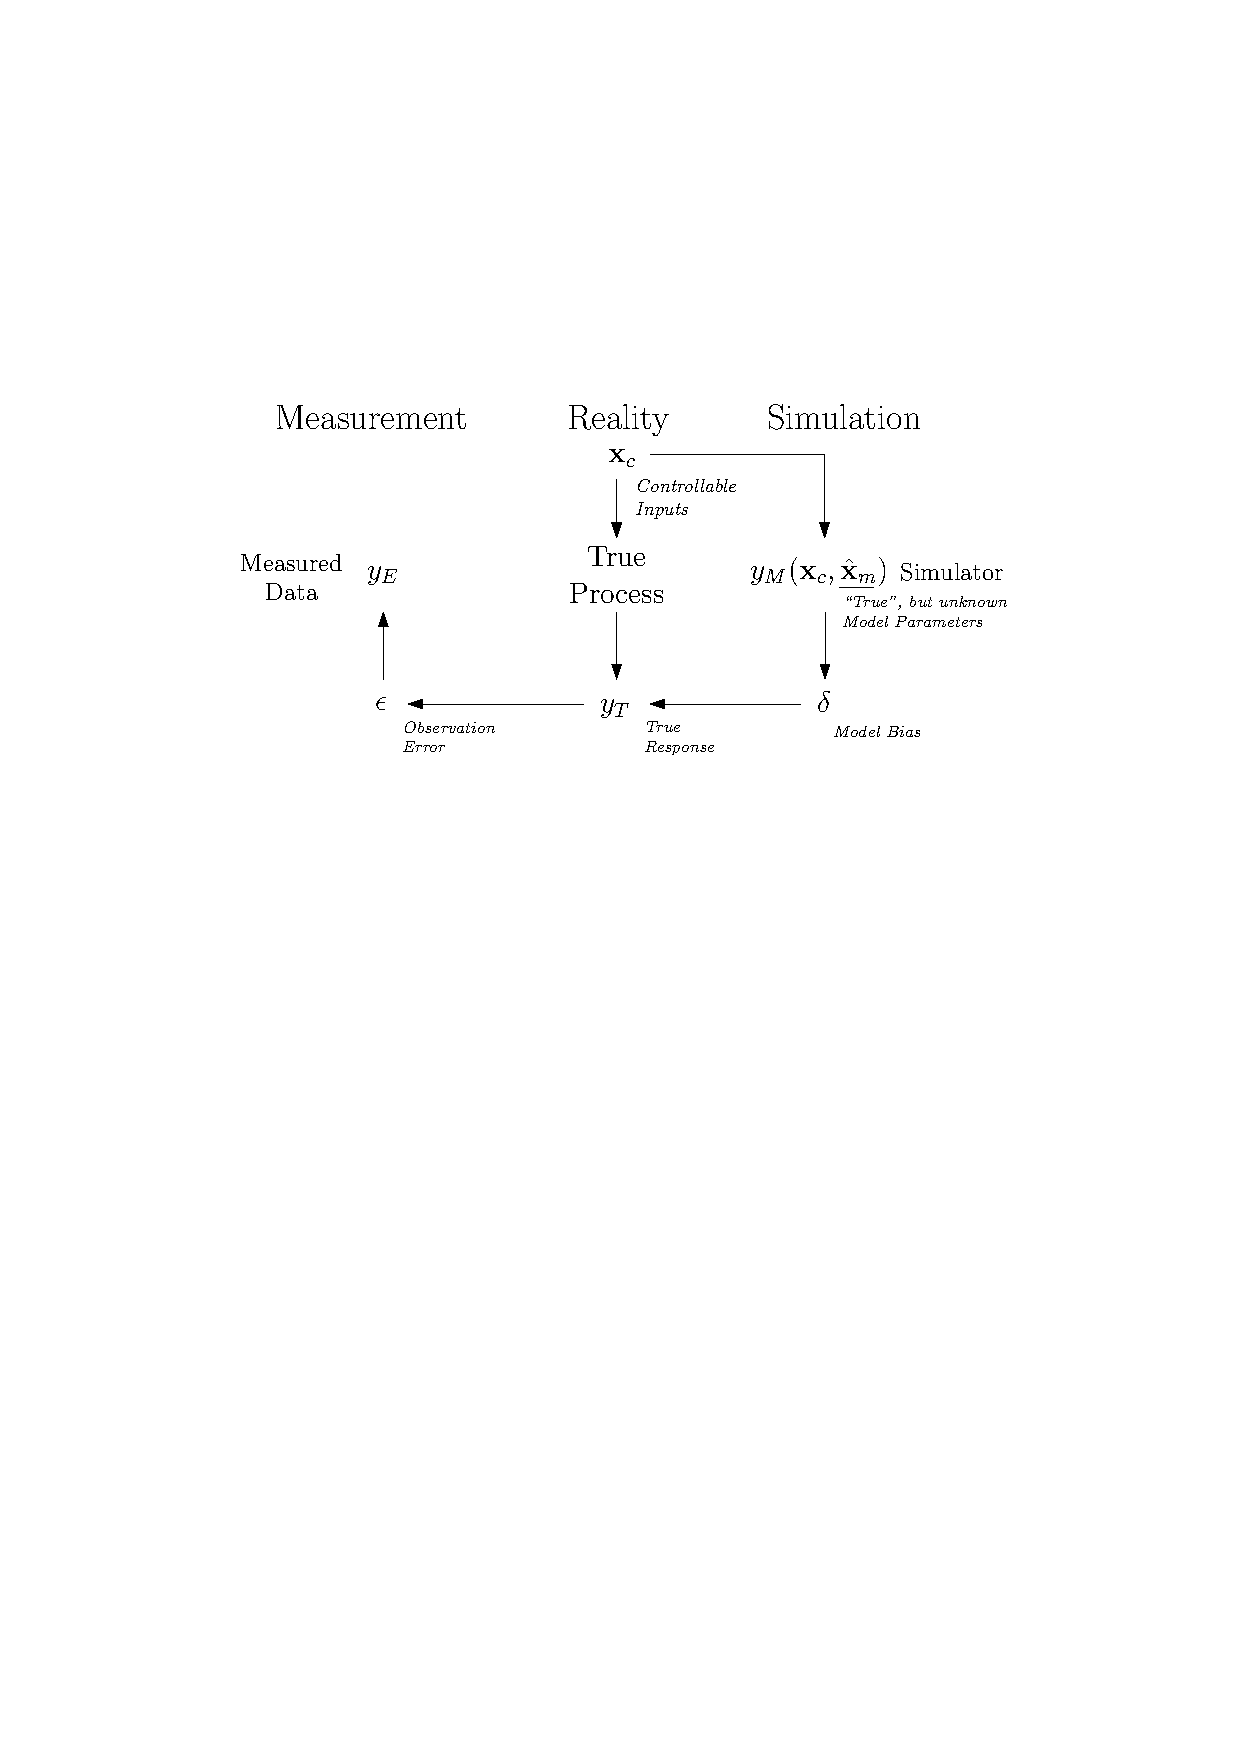
\includegraphics[width=0.91\textwidth]{../figures/chapter5/figures/HMErrorModel}
	\caption[Relationships between elements of the calibration formulation.]{Relationships between elements of the calibration formulation (adapted from \cite{Huard2006}).}
	\label{fig:ch5_hm_error_model}
\end{figure}

% Parametrization, Observation layout
An observation layout, denoted by $\boldsymbol{\Lambda}$, is an ordered set and it defines which of the different types of \gls[hyper=false]{qoi} are observed (or predicted) as well as their locations and time points.
\marginpar{Observation layout}
In this manner, multivariate \glspl[hyper=false]{qoi} can be represented using long vectors \cite{Reichert2012}.
For instance, the observation layout $\boldsymbol{\Lambda} = \{(A,t_1), (B,t_1), (A, t_2)\}$ might be used to signify  \glspl[hyper=false]{qoi} (observed or predicted) of type $A$ at time $t_1$, type $B$ at time $t_1$, and type $A$ at time $t_2$.
The vectors $\bm{y}_M(\circ;\boldsymbol{\lambda})$ and $\bm{y}_E(\circ;\boldsymbol{\lambda})$ for $\boldsymbol{\lambda} \in \boldsymbol{\Lambda}$ then refer to the model prediction and experimental data given by the set, respectively.

% Parameterization, Controllable Parameter
Departing from the previous chapters, this chapter categorically distinguishes two types of input parameters: controllable inputs $\bm{x}_c$ and model parameters $\bm{x}_m$.
\marginpar{Controllable inputs}
Controllable inputs (also known as design variables) are parameters that, in the context of a controlled experiment, can be varied by the experimentalist.
Being controllable also implies that the parameters can be observed in the actual experiment.
In the physical experiment, their values are often varied either to investigate the system behavior under the change or to find the setting that gives the best system performance.
Likewise, in the simulator, controllable inputs are varied by an analyst for the same reasons.
An example of such parameters is the parameters related to boundary conditions of an experiment.

% Parametrization, Model Parameter
Model parameters refer to parameters that are specific to a particular parametrization of the model in the simulator.
As such, they only appear in the term $y_M$ of Eq.~(\ref{eq:bc_observation_true}).
\marginpar{Model parameters}
Model parameters might or might not have a physical meaning;
that is, the parameters have interpretation outside the context of the physical model in which the parameters reside, or the parameters are simply used to tune the model such that the prediction agrees better with the observed data (thus become a measure for model inadequacy of a particular model).
The parameters are referred to as \emph{physical parameters} in the former case,
and as \emph{tuning parameters} in the latter.
In the following, however, such distinction is merely conceptual;
these parameters are in practice not known a priori and not directly observable with respect to the experiment 
As mentioned, the generic goal of model calibration is to obtain an optimal value of the model parameters $\hat{\bm{x}}_m$ based on a set of experimental data taken at particular values of $\bm{x}_c$ and $\bm{\lambda}$.
This distinction will be revisited in Section~\ref{sub:bc_modular_bias}.
The notion of the \emph{true} value is usually reserved for the optimal value of a physical parameter \cite{OHagan2013} and the term \emph{best} or \emph{best-fitting} value is for a tuning parameter \cite{Bayarri2007}.
Contrary to the controllable inputs, once calibrated, model parameters should in principle be valid for all instances of the simulator application.
%Note, however, these two types of parameters are considered simply as input parameters when running the simulator, i.e., $\bm{x} = \{\bm{x}_c, \bm{x}_m\}$.

% Goal of Calibration
The formulation given in Eq.~(\ref{eq:bc_observation_true}) contains two unknowns, namely the best value of the model parameters $\hat{\bm{x}}_m$ and the model bias $\delta$.
\marginpar{Bayesian statistical calibration}
In the Bayesian statistical framework, any unknown is considered \emph{uncertain} and assigned a prior probability distribution.
This prior probability assignment also applies for other terms that might also not be perfectly known, such as the controllable variable $\bm{x}_m$ or the observation error $\epsilon$. 
The goal of calibration is then to update the prior uncertainties on the model parameters based on a comparison between experimental data and simulator prediction.
As such, the calibration process becomes a Bayesian inference.
Consequently, the process takes into account multiple sources of uncertainty in the result.
Appropriately acknowledging multiple sources of uncertainty in the calibration process can provide a hedge against \emph{overfitting}, where the calibrated parameters are overly specific to the data used for the calibration and not applicable in a different setting of controllable inputs.

% Bayesian Data Analysis
Two steps are involved in conducting a Bayesian inference.
\marginpar{Bayesian inference}
The first is a formulation of a full probability model for all the terms in Eq.~(\ref{eq:bc_observation_true}).
In essence, the resulting model represents a data-generating process of the observed experimental data,
incorporating the elements of Eq.~(\ref{eq:bc_observation_true}) into it.
An approach to formulate a full probability model is presented in Section~\ref{sec:bc_modular}.
The full probability model is then conditioned on the given experimental data to obtain an updated (\emph{posterior}) probability distribution of the model parameters.
Dealing with a high-dimensional arbitrary probability distribution is difficult and most of the computations involving  posterior distribution resort to directly generating samples from it. 
Indeed, the computation of the posterior distribution or any transformation of it (e.g., mean of a function) is the second step of the inference and it is presented in Section~\ref{sec:bc_mcmc}.
